\begin{refsection}
\chapter{Further investigations into Ch-bonding at oxygen}\label{sec:o-ch-bonding-further}

\section{Introduction}
Following our initial discovery of unconventional Ch-bonding in \emph{o}-nitro-O-aryl oximes, we sought to establish a structural correlation to bring it in line with the current understanding of Ch-bonding.
To this end, we attempted to manipulate the electron density on both Ch-bond donor and acceptor, and measure the structural changes that result.
We believed that this was important to further substantiate our claim of Ch-bonding being a significant stabilising factor.

\section{Results and discussion}

\subsection{CSD search}

\begin{figure}
    \centering
    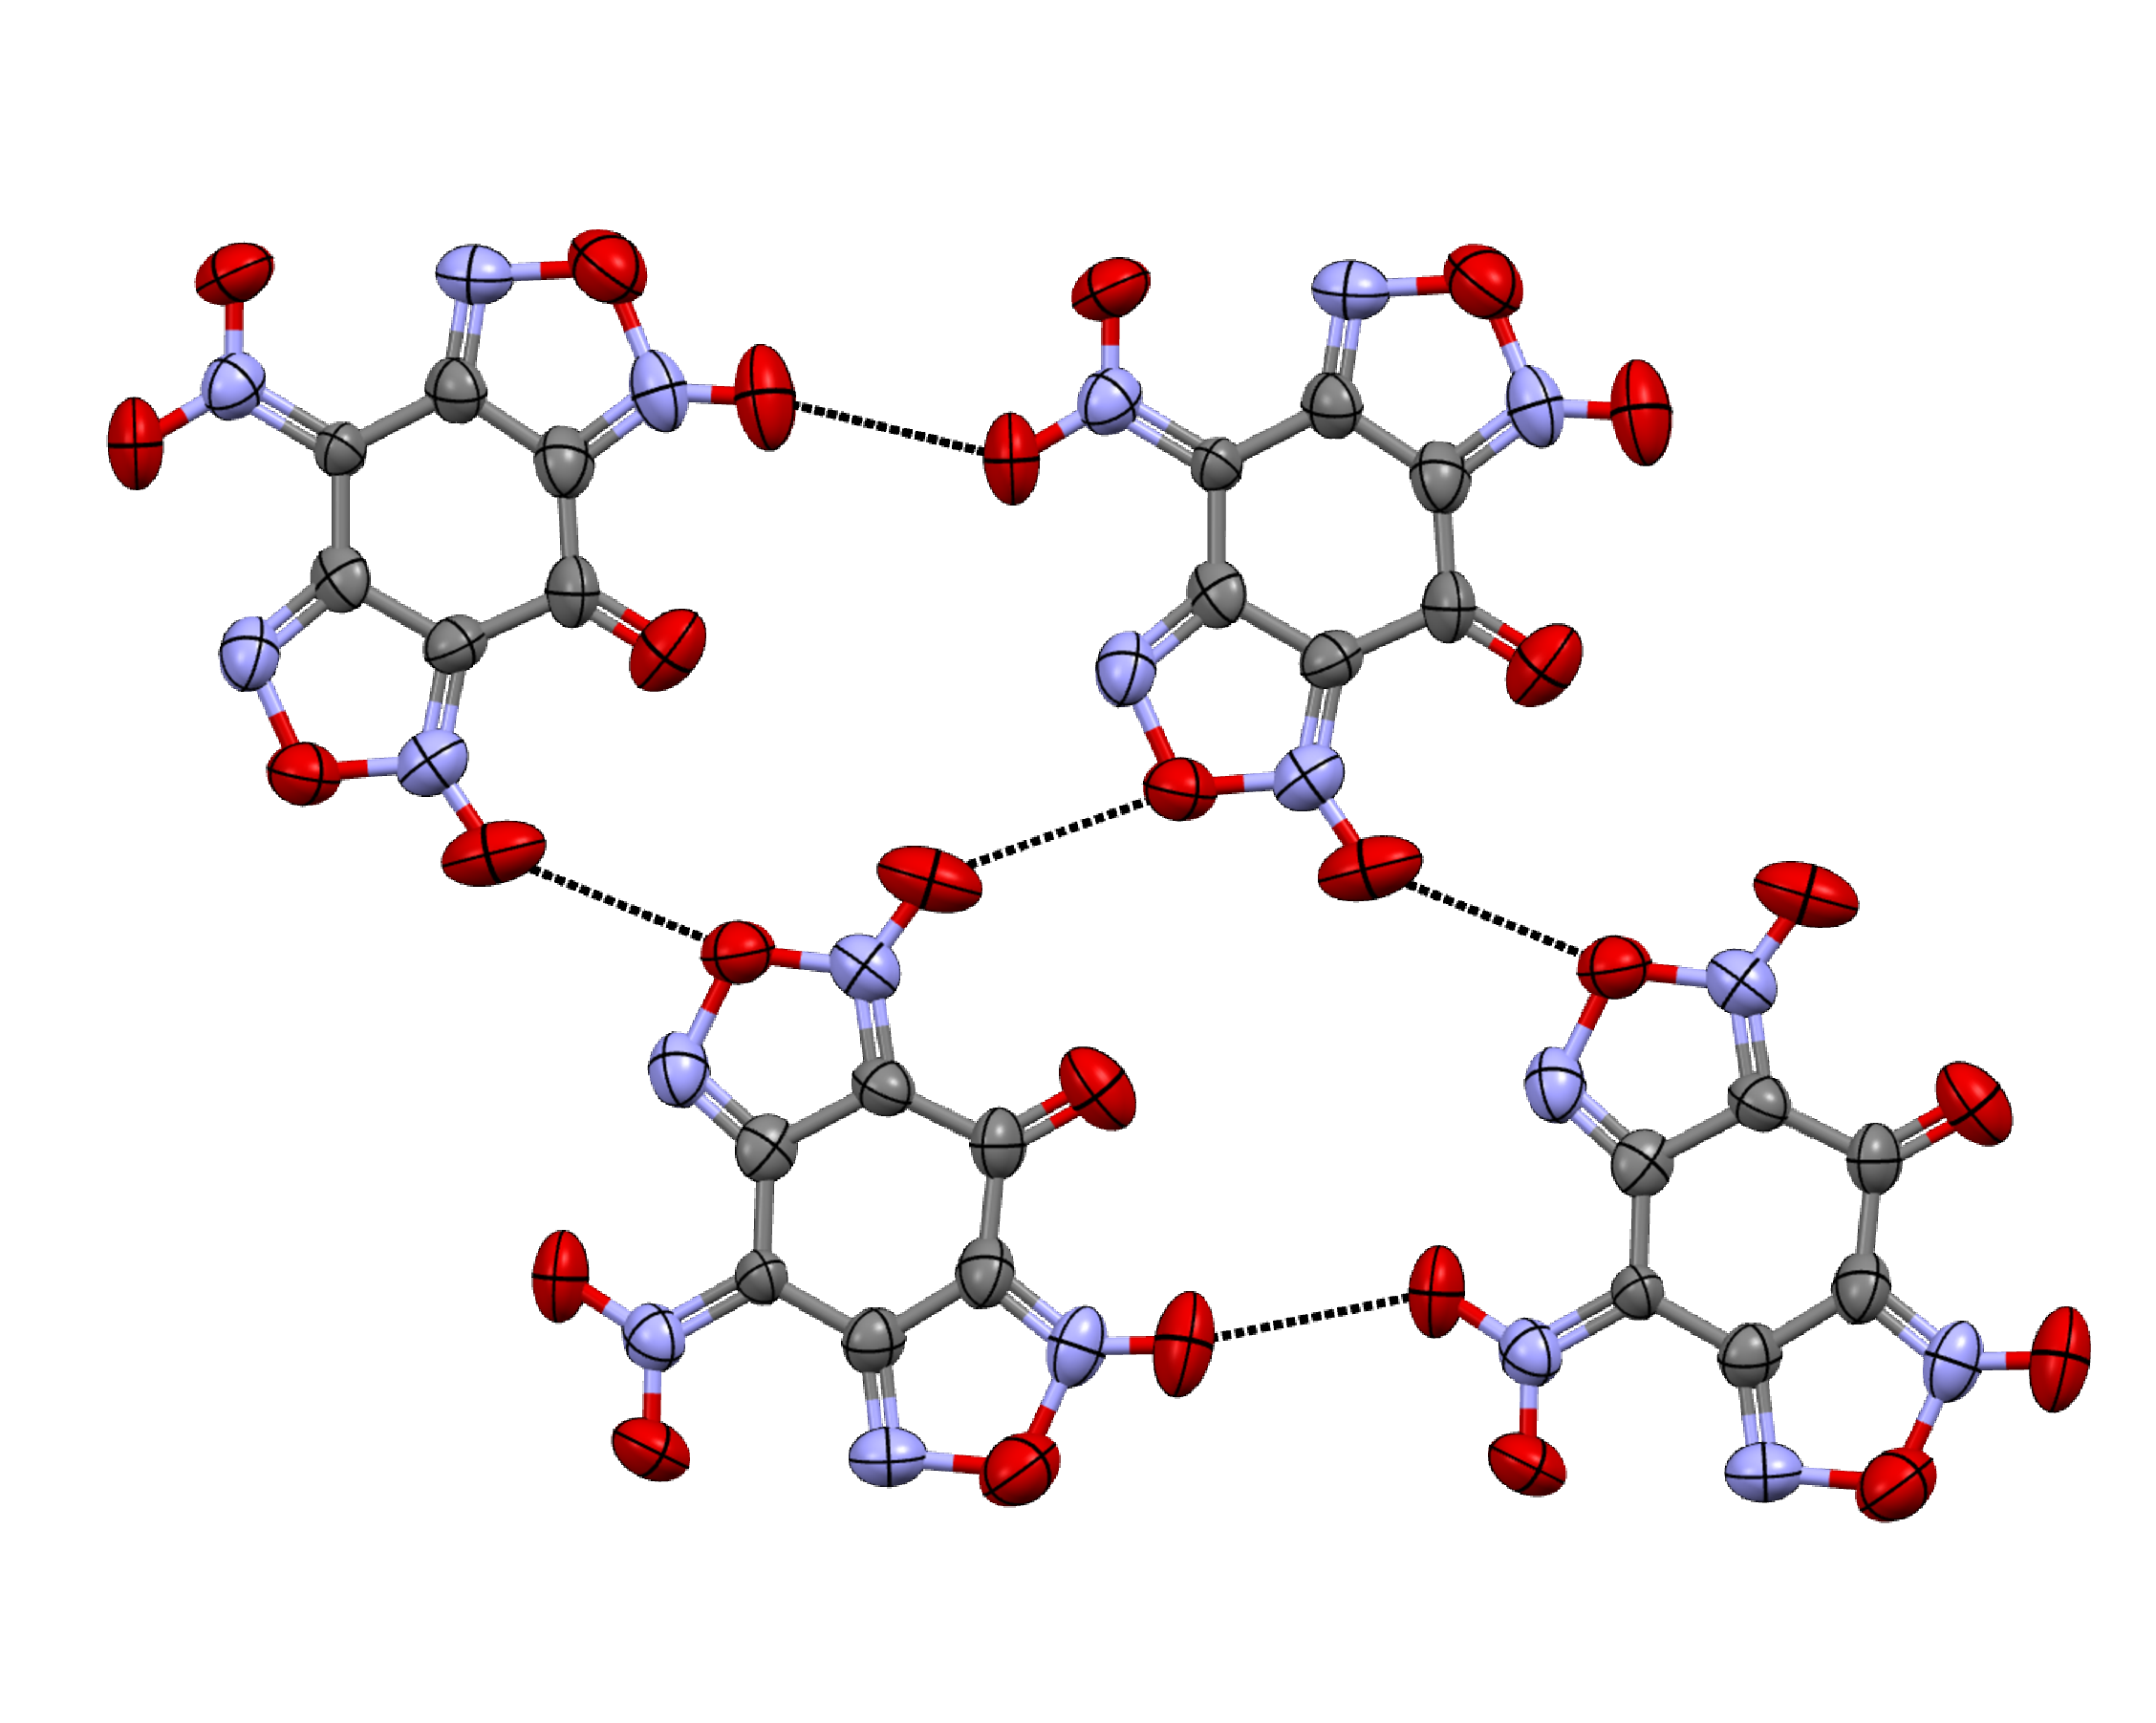
\includegraphics[width=0.45\textwidth]{Figures/XERPOA.pdf}
    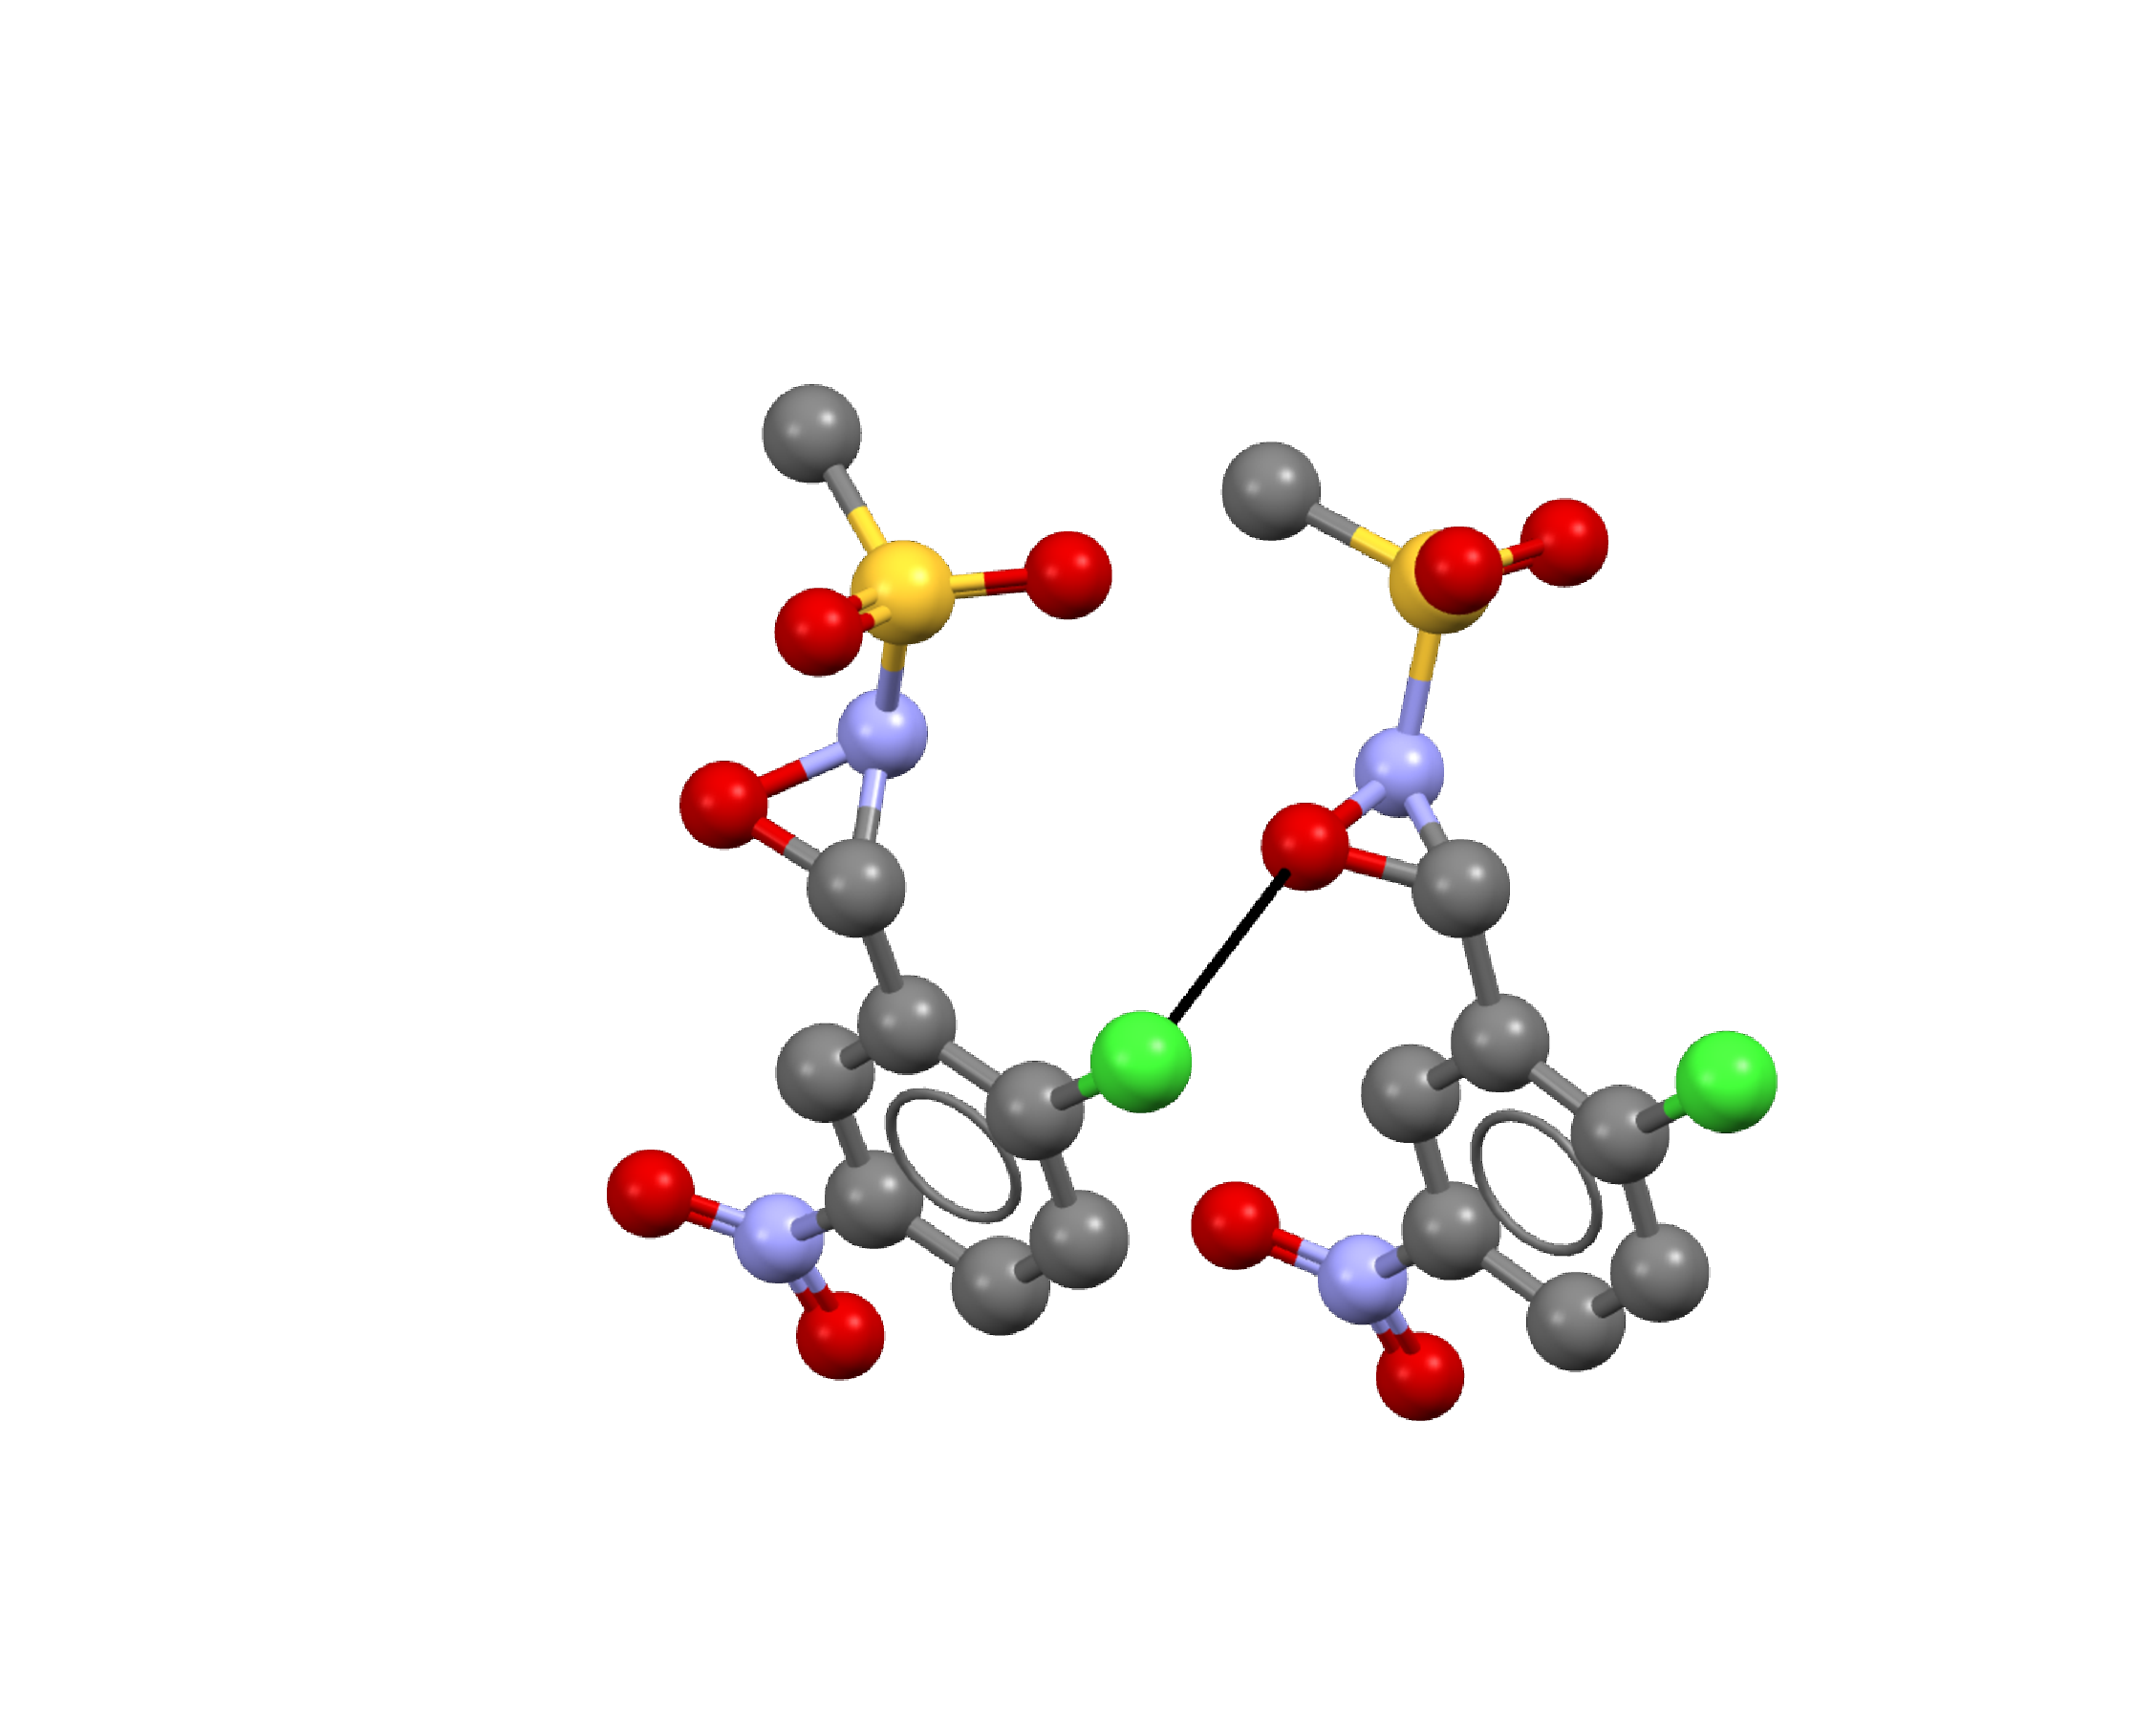
\includegraphics[width=0.45\textwidth]{Figures/FIVJEZ.pdf}
    \caption[Structures of \textbf{XERPOA} and \textbf{FIVJEZ}.]{Structures of \textbf{XERPOA} and \textbf{FIVJEZ} with Ch-bonds indicated by black dotted lines.}\label{fig:furoxan-oxaziridine}
\end{figure}

Since the publication of our first report, we became aware of other apparent Ch-bonds involving oxygen, although they were not initially recognised as such.
Consistent with expectations, they both involve oxygen atoms bonded to nitrogen.
The packing of bis-furoxan \textbf{XERPOA} is directed by intermolecular \ce{O\cdots O} Ch-bonds, although the structure is also stabilised by the \ce{Rb+} counterion (not shown).\autocite{Gilardi2005}
The classic oxaziridine electrophilic oxygen species \textbf{FIVJEZ} also exhibits a Ch-bond between the oxygen and the chlorine on an adjacent molecule.\autocite{Malpezzi1987}
Both structures are shown in \cref{fig:furoxan-oxaziridine}.
The presence of these \emph{inter}molecular Ch-bonds is encouraging, as it indicates that oxygen-based Ch-bonds are competitive with other interactions, and therefore likely to be of interest for the purposes of drug discovery or crystal engineering.\autocite{Taylor2020}

\subsection{Structural studies of analogues}
As the Ch-bond appears to be a primarily electrostatic interaction, it follows that the strength of the Ch-bond will be correlated with the difference in electrostatic potential between the donor and acceptor.

\begin{figure}
    \centering
    \begin{subfigure}{0.45\linewidth}
        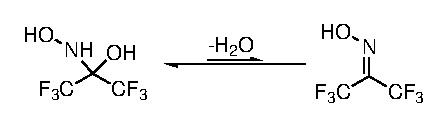
\includegraphics[scale=0.74,trim=0 -1cm 0 -1cm]{Figures/hexafluoroacetone.eps}
    \end{subfigure}
    \begin{subfigure}{0.45\linewidth}
        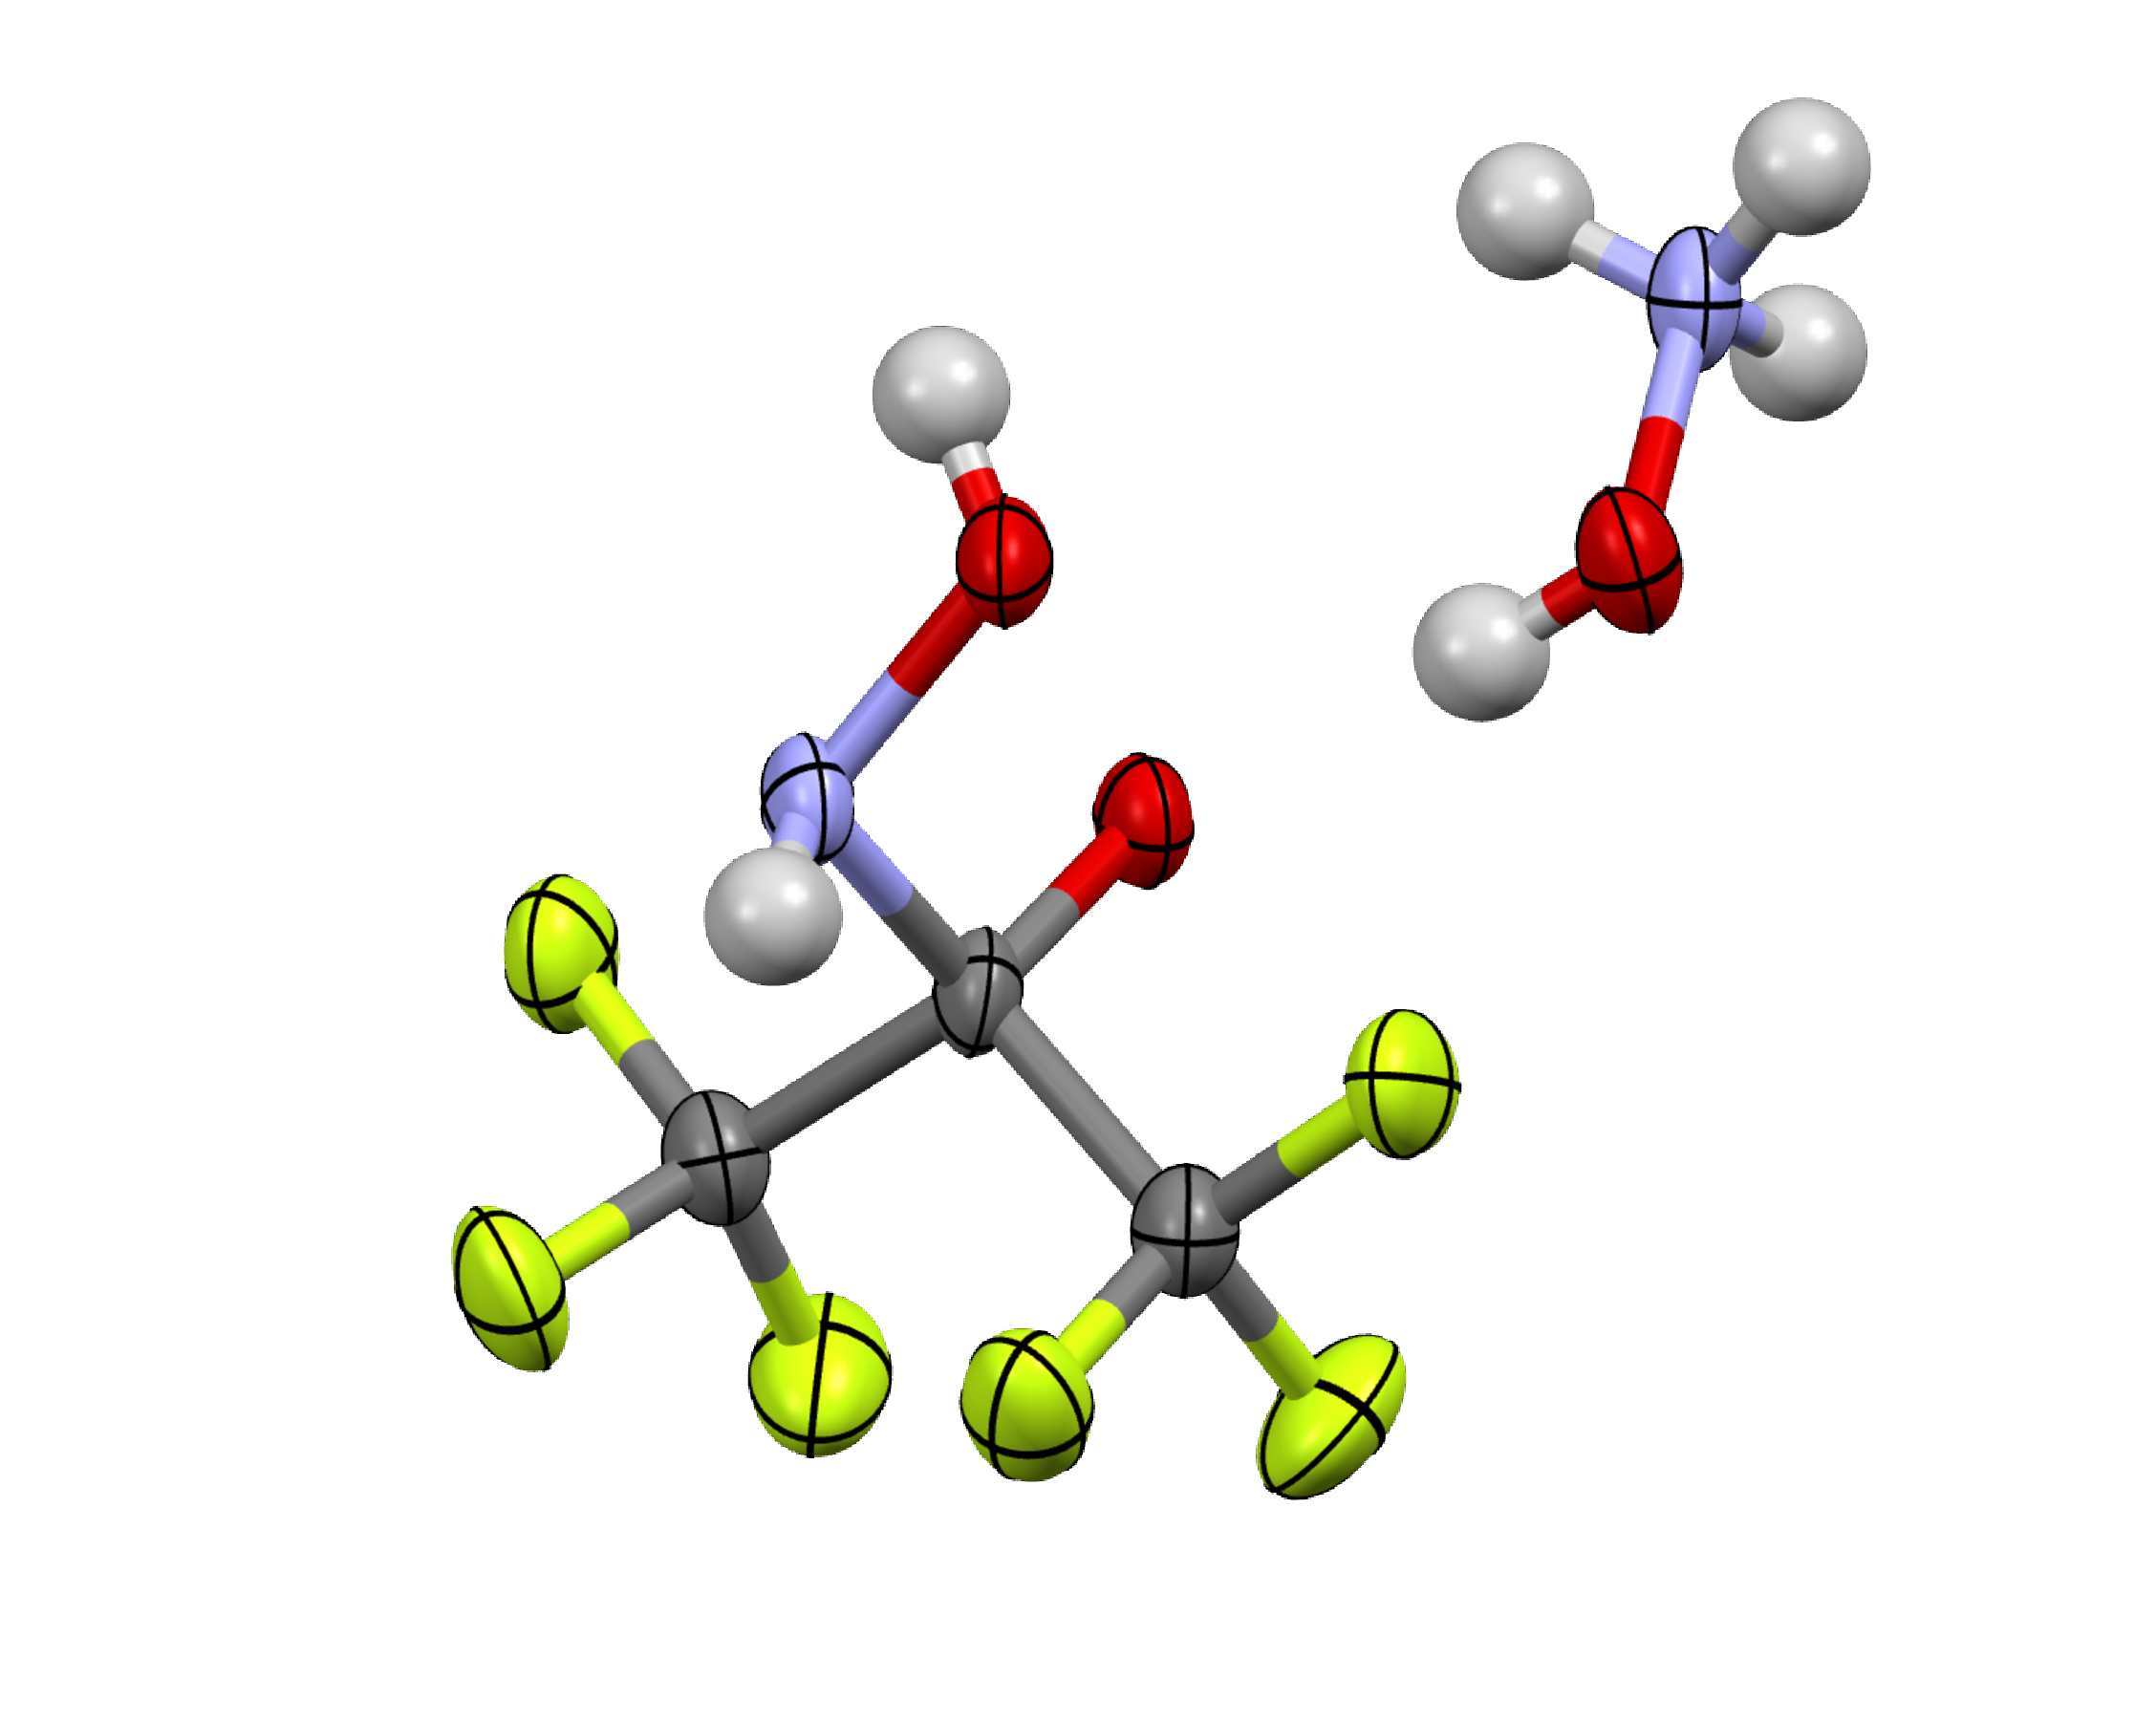
\includegraphics[width=4cm]{Figures/hexafluoroacetone_oxime.pdf}
    \end{subfigure}
    \caption[Dehydration of electron poor hemiaminals.]{The dehydration of electron poor hemiaminals is strongly disfavoured. Instead, the hydroxylammonium salt was isolated as a crystalline solid.}\label{sch:hexafluoroacetone}
\end{figure}

To test this, we synthesised a series of analogues which varied in the electron density at the nitro and oxime groups.
We first attempted to investigate the effects of substantially increasing the electrophilic character of the oxime oxygen, by starting from an electron-poor oxime.
Initial efforts to form hexafluoroacetone oxime (from hexafluoroacetone deuterate and hydroxylamine) were hampered by the fact that the dehydration equilibrium strongly favours the hemiaminal form (\cref{sch:hexafluoroacetone}).

Various methods to remove the water failed, so we persisted with the cyclohexanone oxime (as these derivatives had been shown to crystallise well) and instead modified the electronic properties of the aryl group.

\begin{figure}
    \centering
    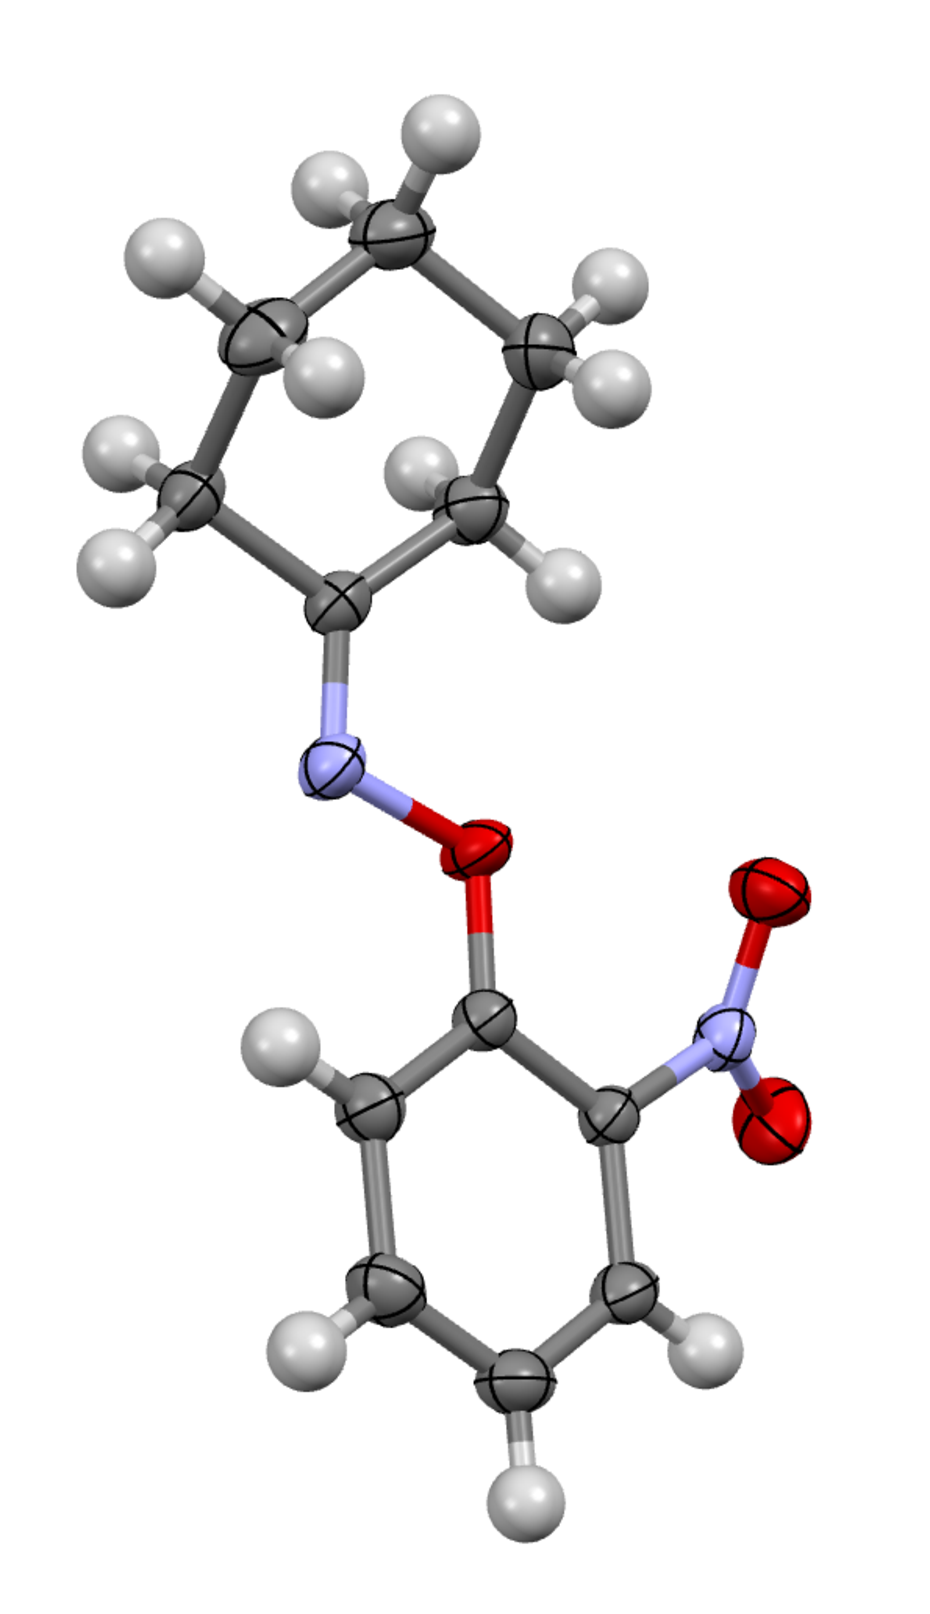
\includegraphics[height=4cm]{Figures/cyclohexanone-oxime-2np.pdf}
    \replacecmpd{cyclohexanone-oxime-2np}
    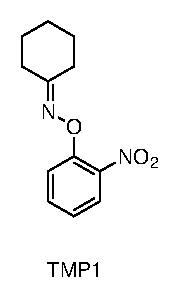
\includegraphics[scale=0.74]{Figures/cyclohexanone-oxime-2np.eps}
    \caption[Structure of \refcmpd{cyclohexanone-oxime-2np}.]{The structure of \refcmpd{cyclohexanone-oxime-2np} exhibits a torsion of the nitro group, suggesting the Ch-bond is too weak to overcome the exchange repulsion between the oxygens.}\label{fig:cyclohexanone-oxime-2np}
\end{figure}    

We first prepared a derivative lacking a nitro group at the 4 position of the aryl ring (compound \cmpd{cyclohexanone-oxime-2np}).
Removing the electron-withdrawing nitro group at this position make the oxime oxygen somewhat more electron rich, while having a negligible effect on the Lewis basicity of the other nitro group.
This has the effect of ``switching off'' the Ch-bond, by reducing its strength relative to other effects.
Indeed, this can be observed in the crystal structure (\cref{fig:cyclohexanone-oxime-2np}), where the nitro group adopts a twisted orientation similar to that of \cmpd{acetone-oxime-dnp}.

\begin{figure}
    \includegraphics[width=0.7\linewidth]{Figures/cyclohexanone-oxime-2np-bcp.png}
    \caption[Bond path and BCP in \refcmpd{cyclohexanone-oxime-2np}.]{Bond path and BCP in \refcmpd{cyclohexanone-oxime-2np}. The BCP is shown in green and the ring critical point in blue.}\label{fig:cyclohexanone-oxime-2np-bcp}
\end{figure}

Interestingly, despite the torsion of the nitro group, a bond path and BCP is still observed (\cref{fig:cyclohexanone-oxime-2np-bcp}).
However, the ring critical point and BCP are separated by only 0.401~\AA\ suggesting that the bond path is actually just a consequence of the proximity of the oxygen atoms.
The bond path is disrupted (the BCP and ring critical point coalesce and annihilate each other) by libration of the nitro group, thus its influence on the energy of the molecule is minimal.\autocite{Farrugia2006}

\begin{figure}
    \centering
    \begin{subfigure}[b]{0.47\linewidth}
        \centering
        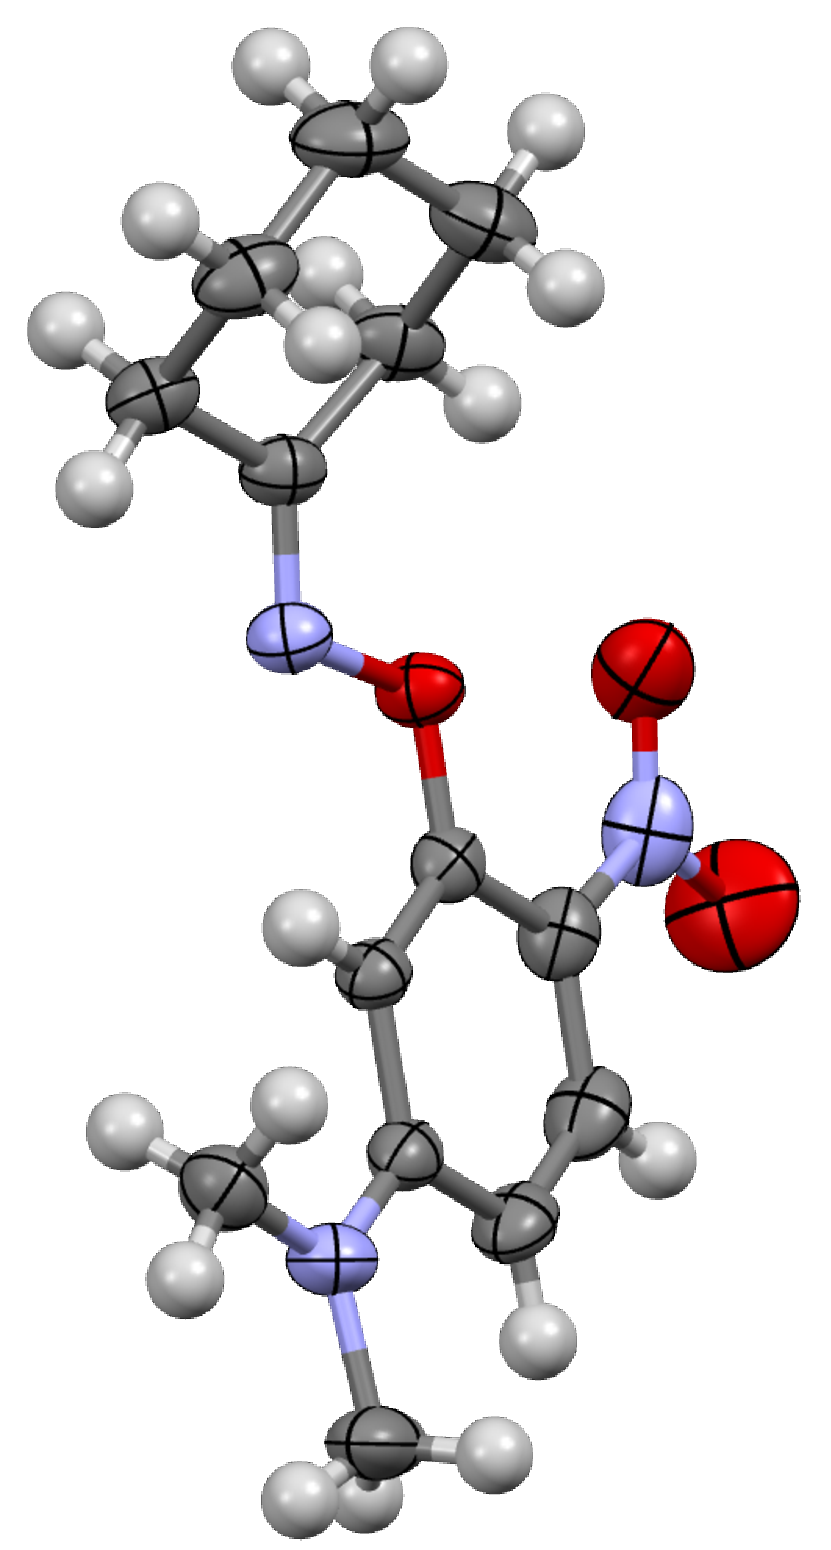
\includegraphics[height=3cm]{Figures/cyclohexanone-oxime-2n-5nme2p.pdf}
        \replacecmpd{cyclohexanone-oxime-2n-5nme2p}
        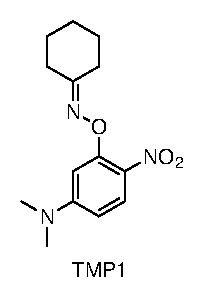
\includegraphics[scale=0.74]{Figures/cyclohexanone-oxime-2n-5nme2p.eps}
        \caption[Structure of \refcmpd{cyclohexanone-oxime-2n-5nme2p}.]{The structure of \refcmpd{cyclohexanone-oxime-2n-5nme2p} features a coplanar nitro group. The increased basicity of the nitro oxygen is sufficient to overcome the repulsion.}\label{fig:cyclohexanone-oxime-2n-5nme2p}
    \end{subfigure}
    \hfill
    \begin{subfigure}[b]{0.47\linewidth}
        \centering
        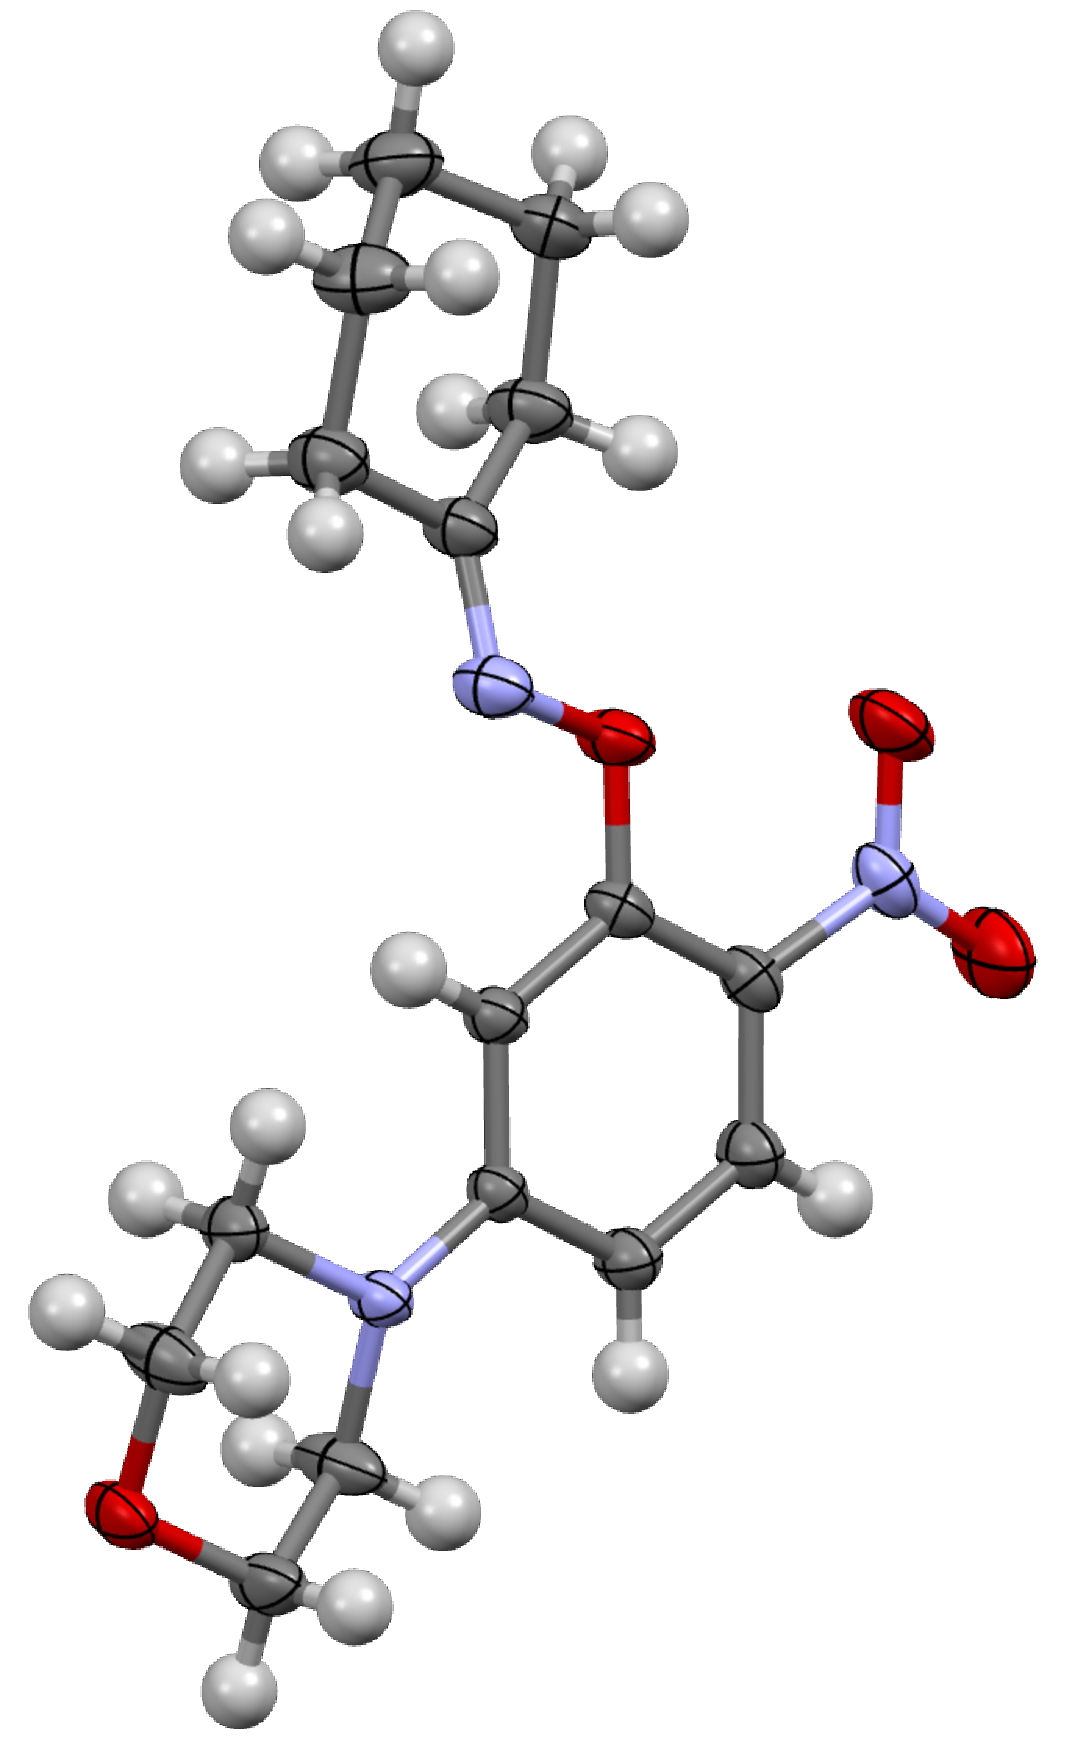
\includegraphics[height=3cm]{Figures/cyclohexanone-oxime-2n-5mpa.pdf}
        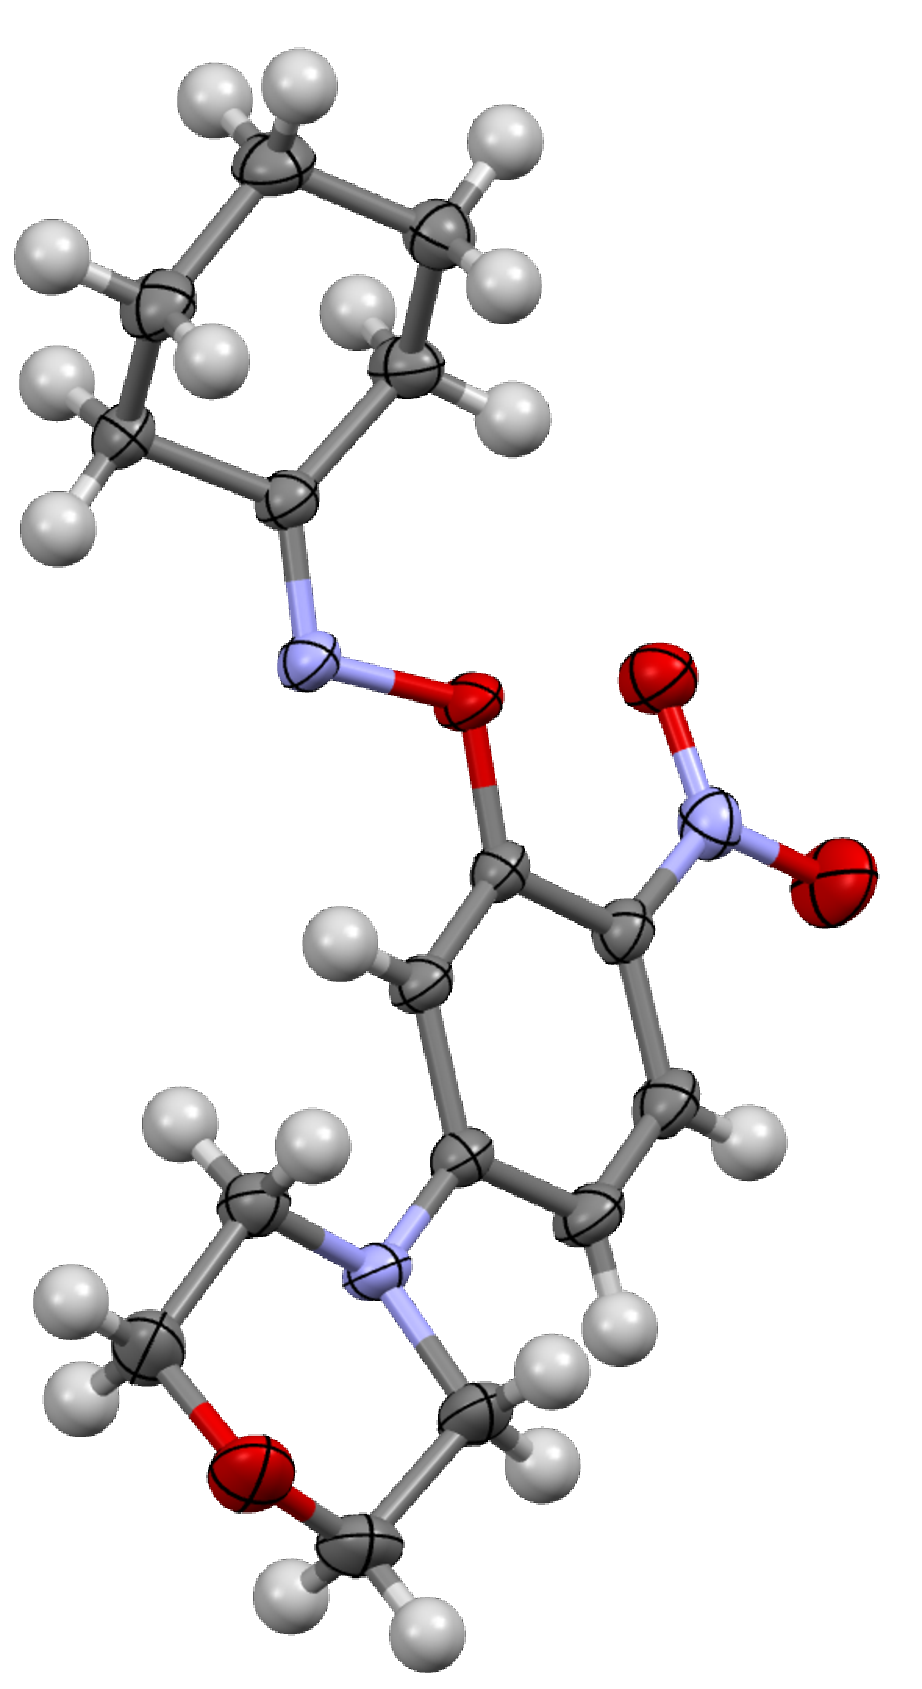
\includegraphics[height=3cm]{Figures/cyclohexanone-oxime-2n-5mpb.pdf}
        \replacecmpd{cyclohexanone-oxime-2n-5mp}
        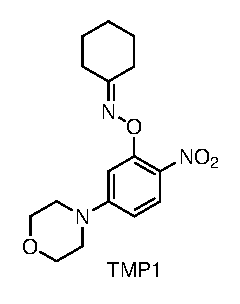
\includegraphics[scale=0.74]{Figures/cyclohexanone-oxime-2n-5mp.eps}
        \caption[Structure of \refcmpd{cyclohexanone-oxime-2n-5mp}.]{The structure of \refcmpd{cyclohexanone-oxime-2n-5mp} also features coplanar nitro groups. There are two molecules in the asymmetric unit, and both are shown.}\label{fig:cyclohexanone-oxime-2n-5mp}
    \end{subfigure}
    \caption[Structures of \refcmpd{cyclohexanone-oxime-2n-5nme2p,cyclohexanone-oxime-2n-5mp}.]{}
\end{figure}

With this encouraging result, we sought to switch the Ch-bond back on again by improving the donor ability of the \emph{o}-nitro group.
This was accomplished by introducing an electron donating group at the 5 position of the ring, which has the effect of increasing electron density at the \emph{o}-nitro group while leaving the oxime relatively unchanged.
Compounds \cmpd{cyclohexanone-oxime-2n-5nme2p,cyclohexanone-oxime-2n-5mp} were prepared, both of which had similar electronic properties (\cref{fig:cyclohexanone-oxime-2n-5nme2p,fig:cyclohexanone-oxime-2n-5mp}).

To our delight, crystals of \cmpd{cyclohexanone-oxime-2n-5nme2p,cyclohexanone-oxime-2n-5mp} showed a coplanar geometry of the nitro group, indicating that Ch-bonding had been switched on again.
Unfortunately, we were unable to obtain crystals of sufficient quality for multipole refinement for either \cmpd{cyclohexanone-oxime-2n-5nme2p} or \cmpd{cyclohexanone-oxime-2n-5mp}, so we are restricted to inferring the presence of a Ch-bond from the geometry of the nitro group.

\begin{table}
    \centering
    \caption[Selected geometric parameters of oximes \refcmpd{cyclohexanone-oxime-dnp,cyclohexanone-oxime-2np,cyclohexanone-oxime-2n-5nme2p,cyclohexanone-oxime-2n-5mp}.]{Selected geometric parameters of oximes \refcmpd{cyclohexanone-oxime-dnp,cyclohexanone-oxime-2np,cyclohexanone-oxime-2n-5nme2p,cyclohexanone-oxime-2n-5mp}. The two geometries in the asymmetric unit of \refcmpd{cyclohexanone-oxime-dnp} and \refcmpd{cyclohexanone-oxime-2n-5mp} are indicated as a and b.}\label{tab:oximes-2}
    \small
    \begin{tabular}{llllll}\toprule
        Compound & r(\ce{O1}$\cdots$\ce{O2}) & r(\ce{N1O1}) & r(\ce{N2O2}) & $\angle$(\ce{O2}$\cdots$\ce{O1N1}) & $\theta$(\ce{C1C2N2O2})\\
        & \AA\ & \AA\ & \AA\ & \degree\ & \degree\  \\\midrule
        \cmpd{cyclohexanone-oxime-dnp}a & 2.5423(8) & 1.4556(7) & 1.2264(9) & 160.56(5) & -0.7(1)	\\
        \cmpd{cyclohexanone-oxime-dnp}b & 2.5522(8) & 1.4522(7) & 1.223(1) 	& 160.29(4) & -0.2(1)	\\
        \cmpd{cyclohexanone-oxime-2np}  & 2.6218(5) & 1.4453(5) & 1.2290(4) & 160.27(3) & 31.93(5)  \\
        \cmpd{cyclohexanone-oxime-2n-5nme2p}&2.5512(6)&1.4444(5)& 1.2322(7) & 159.68(3) & 6.94(8)   \\
        \cmpd{cyclohexanone-oxime-2n-5mp}a&2.5530(7)& 1.4454(7) & 1.2364(6) & 156.48(4) & 1.41(8)   \\
        \cmpd{cyclohexanone-oxime-2n-5mp}b&2.5592(6)& 1.4411(7) & 1.2304(7) & 147.05(3) & -11.86(8) \\\bottomrule
    \end{tabular}
\end{table}

Relevant geometric parameters for the oximes studied are presented in \cref{tab:oximes-2}.
The striking increase in the $\theta$(\ce{C1C2N2O2}) torsion angle of the nitro group is visible in \cmpd{cyclohexanone-oxime-2np}, and the associated increase in the r(\ce{O1}$\cdots$\ce{O2}) Ch-bond distance.
Although the second system in \cmpd{cyclohexanone-oxime-2n-5mp} displays a slight torsion of $-11.86(8)$\degree{}, the r(\ce{O1}$\cdots$\ce{O2}) distance is not substantially increased, suggesting a degree of Ch-bonding is still occurring.

As mentioned in \cref{sec:o-ch-bonding}, it is difficult to assess whether the oxime \ce{O-N} bond is lengthened due to the influence of the electronic properties of the phenyl group on this bond length.
However, using the structural correlation \cref{eqn:scp} and the pK\textsubscript{a} of the parent phenol, we can derive an expected value for the bond length.\autocite{Yeoh2012,Socrates1970}
For \cmpd{cyclohexanone-oxime-2np}, the expected oxime bond length is 1.4442~\AA, which is not significantly different to the measured distance of the 1.4453(5)~\AA\ ($\Delta = 0.0011$~\AA~$= 2.2\sigma$).
This supports our assertion that Ch-bonding is not occurring in this derivative, due to the slightly more electron rich oxime.

Although experimental pK\textsubscript{a} values for \cmpd{cyclohexanone-oxime-2n-5nme2p,cyclohexanone-oxime-2n-5mp} are not available, they can be estimated using the Hammett equation and a reaction constant of $\rho=2$ for phenols.\autocite{Hansch1991}
The pK\textsubscript{a} thus calculated for \cmpd{cyclohexanone-oxime-2n-5nme2p} is 7.53, which affords an expected bond length of 1.4429~\AA.
The pK\textsubscript{a} and expected bond length for \cmpd{cyclohexanone-oxime-2n-5mp} is likely to be almost the same.
The measured bond distances of 1.4444(5) and 1.4454(7)~\AA\ are significantly longer than expected ($\Delta = 0.0015$~\AA~$= 3\sigma$ and $\Delta = 0.0025$~\AA~$= 3.6\sigma$), which is again consistent with our claim of Ch-bonding.

\section{Conclusion}

In conclusion, we have shown that the \ce{O\cdots O } contact in \textit{o}-nitro-O-aryl oximes displays structural features consistent with a Ch-bond.
By manipulating the electron density at both the Ch-bond donor and acceptor, we are able to turn the Ch-bond on and off.
This is manifested in varying degrees of torsion of the nitro group, as the balance between exchange repulsion and electrostatic attraction due to the $\sigma$-hole shifts.

\section{Supplementary material}

\subsection{Synthesis}

\subsubsection[Preparation of \refcmpd{cyclohexanone-oxime-2np,cyclohexanone-oxime-2n-5nme2p,cyclohexanone-oxime-2n-5mp}]{Preparation of \emph{O}-(2,4-dinitrophenyl) oximes \refcmpd{cyclohexanone-oxime-2np,cyclohexanone-oxime-2n-5nme2p,cyclohexanone-oxime-2n-5mp}}
???

\cmpd{cyclohexanone-oxime-2n-5mp}
\ce{^{1}H} NMR (499~MHz, \ce{CDCl3}) $\delta$ ppm 8.04 (1H, d, \textit{J} = 9.32~Hz), 7.16 (1H, d, \textit{J} = 2.41~Hz), 6.45 (1H, dd, \textit{J}\textsubscript{1} = 2.58~Hz, \textit{J}\textsubscript{2} = 9.41~Hz), 3.86 (4H, t, \textit{J} = 4.71~Hz), 3.37 (4H, t, \textit{J} = 4.78~Hz), 2.82 (2H, t, \textit{J} = 6.36~Hz), 2.5 (1H, t, \textit{J} = 6.03~Hz), 2.39 (2H, t, \textit{J} = 6.19~Hz), 2.21 (1H, t, \textit{J} = 6.35~Hz), 1.85--1.71 (4H, m).

\printbibliography[heading=subbibliography]
\end{refsection}